\chapter{Grundlagen}\label{ch:basics}

\section{Übungskonzept}\label{sec:programming-assignments}

Der Anwendungsfall dieser Arbeit umfasst den gesamten Lebenszyklus einer Hausaufgabe als Teil einer Lehrveranstaltung.
Dieser besteht aus mehreren zeitlichen getrennten Phasen, die nachfolgend beschrieben werden.
Abschnitt~\ref{subsec:workflow} betrachtet den Ablauf, um die Hintergründe und zu lösende Probleme des zu entwickelnden Werkzeugs zu verdeutlichen.
Verschiedene Parteien nehmen an dem Übungsablauf teil.
Ein Professor oder Mitarbeiter oder eine Professorin oder Mitarbeiterin, nachfolgend zusammegefasst als Übungsleitung bezeichnet, steuert den Übungsbetrieb.
Ihre Tätigkeit ist hauptsächlich didaktischer und organisatorischer Natur und wird durch das Werkzeug dieser Arbeit nur begrenzt unterstützt, weshalb sie im Folgenden nicht weiter diskutiert werden.
Studierende bearbeiten Aufgaben und erzeugen Abgaben, um einen Lernerfolg mit praktischer Anwendung zu erzielen.
Sie werden in Abschnitt~\ref{subsec:students} näher beschrieben.
Für die Leistungseinschätzung von Studierenden sind Betreuende zuständig, welche die Abgaben gegen zuvor festgelegte Kriterien bewerten und dabei eine Punktzahl ermitteln und vergeben.
Betreuung und Übungsleitung müssen nicht zwangsläufig verschiedene Personen sein, bei einer großen Anzahl von Studierenden werden jedoch aus Zeitgründen weitere Mitarbeitende oder Hilfskräfte mit der Bewertung beauftragt.
Details zu dieser Personen- und Benutzergruppe werden in Abschnitt~\ref{subsec:teaching-assistants} diskutiert.

\subsection{Ablauf}\label{subsec:workflow}

Der Ablauf oder Lebenszyklus einer Hausaufgabe im Übungsbetrieb besteht für die Zwecke dieser Arbeit aus vier Phasen unterschiedlicher Länge:
Konzeption, Vergabe, Bearbeitung, und Bewertung.
Diese werden nachfolgend näher definiert und beschrieben.

Es ist üblich, dass bei regelmäßiger Hausaufgabenvergabe die Phasen mehrerer unterschiedlicher Hausaufgaben überlappen.
Abbildung~\ref{fig:overlapping-phases} zeigt eine kalendarische Beispielansicht, die diesen Sachverhalt visualisiert.
In diesem Beispiel sind je vier Tage für Konzeptionsphase vorgesehen und die Bearbeitungsfrist und Bewertungszeit beträgt jeweils eine Woche.
Dabei ist zu erkennen, dass ab der zweiten Woche an jedem Tag mindestens zwei Phasen gleichzeitig verlaufen.
Am Anfang jeder Woche ist sichtbar, dass Bewertung und Konzeption gleichzeitig stattfinden.
Folglich ist wie zuvor genannt sinnvoll, dass unterschiedlichen Personen diese beiden Phasen durchführen.

\begin{figure}
    \centering
    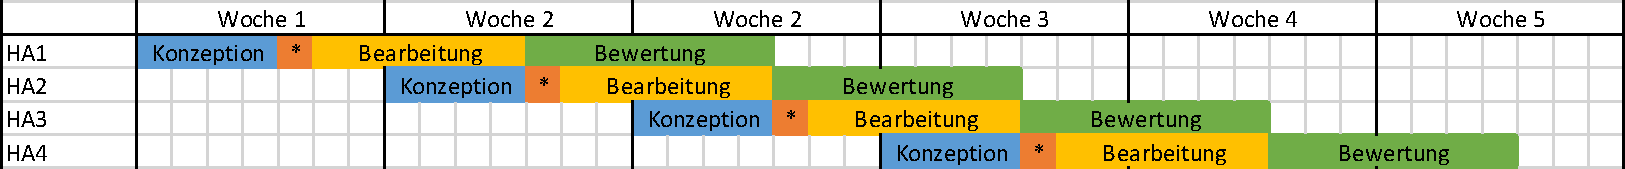
\includegraphics[width=\textwidth]{images/ablauf}
    \caption{Übersicht des Ablaufs und Überlappung von Hausaufgabenphasen. \textbf{*} markiert den Tag der Vergabe und damit den Beginn der Bearbeitungszeit.}
    \label{fig:overlapping-phases}
\end{figure}

\subsubsection{Konzeption}

Die Konzeptionsphase umfasst die Erstellung der Aufgabenstellung, in Berechnung und Vergabe der Punktzahlen und einhergehende Erstellung von Bewertungsrichtlinien, sowie bedingt die Erstellung einer Musterlösung.
Die Aufgabenstellung entsteht meist in Anlehnung an die in der Vorlesung vermittelten Lehrinhalte, um diese bei Lernenden zu stärken.
Alternativ kann die Übung einen eigenen Lehrplan verfolgen und von der Vorlesung unabhängig ablaufen.
In beiden Fällen müssen die Aufgaben selbst und eventuell notwendige Zusatzinformationen, darunter beispielsweise die Abgabemodalitäten oder Kontaktangaben für Rückfragen, verschriftlicht werden.
Es handelt sich dabei größtenteils um einen kreativen und nicht repetitiven Prozess, dessen Automatisierung oder Unterstützung nicht von dieser Arbeit erstrebt wird.
Um die Forschungsfrage RQ4 zu erklären, ist es jedoch notwendig zu untersuchen, ob bereits in dieser Phase Anpassungen vorgenommen werden können, um die nachfolgenden Phasen zu vereinfachen.
Ebenfalls interessant ist der Einfluss einer Musterlösung, welche zwar zu einem zeitlichen Mehraufwand bei der Konzeption führen kann, aber möglicherweise Vorteile in späteren Schritten hervorrufen kann.
Nicht zuletzt kann eine Musterlösung helfen, die Erfüllbarkeit der Aufgaben zu überprüfen oder eine Demonstration als Teil der Vergabe zu ermöglichen.

\subsubsection{Vergabe}

Die Vergabe bezeichnet den Zeitpunkt, an dem die Aufgabenstellung an die Studierenden veröffentlicht wird.
Mit deren Einsicht beginnt für Gewöhnlich die Bearbeitungszeit, da Vorüberlegungen und Umsetzungsgedanken getroffen werden können.
Die Vergabe ist folglich gleichzusetzen mit dem Beginn der Bearbeitungszeit.
Es bietet sich an, die Vergabe während der Übungsveranstaltung durchzuführen.
Dabei können die Aufgaben gezeigt und erklärende Bemerkungen gemacht werden.
Dies ist jedoch nicht zwingend erfordlich, sofern der Text selbst ausreichend detailliert die Aufgabe beschreibt.
Weiterhin kann hier eine Demonstration der in der Aufgabe gefordeten Lernziele gemacht werden.
Dabei kann das gewünschte Endergebnis oder Quellcode gezeigt werden, sofern letzterer ausreichend angepasst wurde, um nicht die Lösung vorwegzunehmen.
Ein angepasstes Beispiel kann in diesem Fall die Transferleistung erlauben.

\subsubsection{Bearbeitung}

Die Bearbeitungsphase ist zeitlich genau durch die Vergabe und die Abgabefrist beschränkt.
Während dieser Zeit sollen Studierende die Aufgabenstellung lesen, verstehen und befolgen, um bis Ablauf der Frist eine fertige Abgabe zu erstellen.
Dabei ist tatsächliche Bearbeitungsdauer für jeden Studierenden unterschiedlich, abhängig von dessen generellem Verständnis für das Fach, eventuelle Vorerfahrung und Affinität bei der Umsetzung.
Die Form der Abgabe kann abhängig von der Aufgabenstellung und Veranstaltung stark variieren.
Denkbar sind handschriftliche Abgaben in Papierform, digitale Textdateien, Scans oder sonstige Dokumente, oder Quellcode in Form einzelner Dateien oder Projekte.
Bei digitalen Abgaben kann sich weiterhin der Transfer der Abgabe unterscheiden.
Beispiele dafür sind Versand per Email, Hochladen in einen Cloud-Ordner, Lernplatformen wie Moodle\footnote{\url{https://moodle.org/}}, eigene Abgabesysteme oder GitHub Classroom\footnote{\url{https://classroom.github.com/}}.
In dieser Arbeit wird davon ausgegangen, dass nur Quellcode und Textdateien erstellt und über dateibasierte Abgabesysteme oder GitHub Classroom eingereicht werden.

\subsubsection{Bewertung}

Die Bewertungsphase beginnt nach Erreichen der Abgabefrist und ist meist nicht zeitlich beschränkt.
Es ist jedoch, eine Bewertung einer Hausaufgabe vor Abgabefrist der darauffolgenden Hausaufgabe abzuschließen, um die Anhäufung von Arbeit zu vermeiden.
Auch in dieser Phase ist die tatsächliche Dauer von verschiedenen Faktoren abhängig.
Darunter fällt die Anzahl der Abgaben und Bewerter, die parallel bewerten können, sowie deren Affinität.
Des Umfang der Aufgabenstellung kann ebenfalls proportional Einfluss auf die Bewertungsdauer haben.
Zudem ist der Anteil der unvollständigen oder fehlerhaften Abgaben entscheidend, welche einerseits die gänzliche Überspringung von Teilaufgaben, andererseits die umfangreiche Bereitstellung von Erklärungen erfordern können.

Der Ablauf der Bewertung kann durch wenige Schritten beschrieben werden.
Sie beginnt im Fall einer Bewertendenanzahl größer eins mit der Zuteilung von Abgaben oder Teilaufgaben auf die Bewertenden.
Dabei gibt es grundsätzlich zwei Verfahren.
Bei der Teilaufgaben-Verteilung wird jedem Betreuenden eine Teilaufgabe zugewiesen, für die er oder sie alle Abgaben betrachtet, eine Teilpunktzahl berechnet und Begründungen oder Erklärungen in Form von Feedback bereitstellt.
Danach werden alle Teilpunkte zusammengetragen und das Feedback an die Studierenden verteilt.
Dieses Verfahren hat die Vorteile, dass jeder Betreuende nur eine Teilaufgabe kennen und verstehen muss und Plagiate erkennen kann.
Nachteile sind jedoch der erhöhte Aufwand durch die Berechnung der Gesamtpunktzahl und Zusammenführung des Feedbacks, die möglichen Unterschiede im Zeitaufwand der Teilaufgaben, und der fehlende Zusammenhang bei aufeinander aufbauenden Aufgaben.
Aus diesem Grund wird nachfolgend nur noch das zweite Verfahren, die Aufteilung von Abgaben, betrachtet.
Dabei werden jedem Betreuenden eine bestimmte Anzahl von Abgaben zugewiesen, die vollständig bewertet werden müssen.
Der Ablauf ist dann für jede Abgabe gleich - zunächst wird die Lösung betrachtet, dabei werden Punkte und Feedback zusammengetragen, und zuletzt werden beide an den Studierenden versandt.
Auch der Transfer des Feedbacks kann verschiedene Formen, abhängig vom Abgabemechanismus, annehmen.
Beispiele hierfür wären das Feedback per Email, Pull Requests oder Issues auf GitHub, oder Kommentarfunktionen auf Moodle oder anderen Abgabesystemen.

Bei der Bewertung handelt es sich meist um eine repetitive Tätigkeit, da eine Vielzahl von Studierenden die gleiche Aufgabe bearbeitet und somit größtenteils ähnliche Lösungen produziert hat.
Darüber hinaus erfordert die korrekte Berechnung einer Punktzahl für eine Abgabe die Summierung der Punkte aller Teilaufgaben.
Diese rechnerische Tätigkeit kann bei vielen Teilaufgaben zu Rechenfehlern führen, die meist von Studierenden bemerkt und beanstandet werden.
Das Zusammentragen von Feedback und Punktzahl und deren Versand verursachen einen vergleichsweise geringen Zeitaufwand, der sich jedoch bei einer großen Anzahl von Abgaben summieren kann.

\subsection{Studierende}\label{subsec:students}

\todo{
    Kreative Lösungsansätze oder Nachprogrammieren der Vorlesung.
}

\subsection{Betreuende}\label{subsec:teaching-assistants}

\todo{
    Viele Bewertungen am Stück oder nach und nach.
    Akribische Fehlersuche oder flüchtiges Betrachten.
}

\section{Technologien}\label{sec:tech}

Die Implementierung dieser Arbeit basiert in großen Teilen auf der Weiterentwicklung von bestehenden Projekten sowie der Neuentwicklung eines Werkzeugs.
Diese verwenden verschiedene Technologien von Dritten, die nachfolgend beschrieben werden.
In den folgenden Abschnitten wird erläutert, welche Probleme diese Technologien im Kontext des Vorhabens lösen, welche nützlichen Funktionen sie bereitsstellen, und welche Gründe für die Auswahl dieser Technologien bestanden.

\subsection{fulib.org}\label{subsec:fulib.org}

fulib.org ist eine Webanwendung, die bereits 2019 im Rahmen des fulibScenarios-Projekts~\cite{explain} konzipiert und durch~\cite{bachelor-thesis} erweitert wurde.
Sie besteht aus einigen Modulen, die nachfolgend kurz beschrieben werden.

\subsubsection{Scenarios}
Das erste Modul der Anwendung ist ein interaktiver Editor für die Szenario-Sprache aus~\cite{explain}.
Diese besteht aus textuellen Beispielszenarien, die einer festen Grammatik folgen.
Ein Compiler übersetzt die Szenarien in Java-Code und generiert dabei Klassen für ein Datenmodell mit~\cite{fulib}.
In~\cite{bachelor-thesis} wurde erstmals eine Erweiterung der Sprache umgesetzt, die gezielt die Bewertung von Aufgaben ermöglichen sollte.
Dafür wurde spezielle Syntax zur Mustererkennung auf Objektstrukturen entwickelt, die besonders für Fälle geeignet war, in der die Benennung von Variablen, Attributen und Assoziationen nicht festgelegt war.
Nachfolgend werden die Szenario-Sprache und der Editor nicht weiter betrachtet.
Es handelt sich jedoch um wichtige Hintergründe und Erkenntnisse, die in den Abschnitten~\ref{sec:expanding-fulib.org} und~\ref{sec:renaming-and-refactoring} wieder aufgegriffen werden.

\subsubsection{Docs}
Hier kann die Dokumentation für verwandte Werkzeuge aus dem fulib-Toolkit nachgelesen werden.
Diese wird direkt von den jeweiligen GitHub-Repositories bezogen, ist also nicht Teil der Webanwendung selber.
Insbesondere befindet sich hier das Benutzerhandbuch von fulibFeedback.

\subsubsection{Projects}
Dieser Teil der Webanwendung ist eine Prototyp für eine Online-\ac{ide}.
Dort können Projekte erstellt werden, die im Gegensatz zum Szenario-Editor mehrere Dateien umfassen können.
Insbesondere können hier Gradle- und Java-Dateien betrachtet und bearbeitet werden.
Ein Dateibaum zeigt Ordner und darin befindliche Dateien jeglicher Art.
Mit einem Web-Terminal können beliebige Kommandozeilenbefehle ausgeführt werden, darunter auch die zum Bauen und Ausführen verwendeten Gradle-Befehle.
Die Projekte ermöglichen folglich eine eingeschränkte Form der Anwendungsentwicklung in einer Desktop-\ac{ide}.
Nachfolgend werden Projekte nicht weiter eingesetzt, sie bieten sich jedoch für zukünftige Erweiterungen in Abschnitt~\ref{sec:future-projects} an.

\subsubsection{Assignments}
Das ursprünglich in~\cite{bachelor-thesis} entwickelte Assignments-Modul von fulib.org ist nun erneut Zentrum der Implementierung.
In Abschnitt~\ref{sec:expanding-fulib.org} wird vermehrt beleuchtet, welche Änderungen vorgenommen wurden.
Nun soll zunächst beschrieben werden, wie der Stand des Moduls gegen Ende von~\cite{bachelor-thesis} war.
Vor dieser Arbeit waren die Assignments, eine eigene Bezeichnung für Hausaufgabenblätter, nur auf Aufgaben in der Szenario-Sprache fokussiert.
Mit einfachen Formularen konnten Titel, Beschreibung, Abgabefrist und einige Teilaufgaben definiert werden.
Jede Teilaufgabe bestand mindestens aus Kurzbeschriebung und Punktzahl
Optional konnte eine Teilaufgabe mit Verifizierungscode in der Szenario-Sprache, meist mit der Pattern Matching-Syntax aus~\cite{bachelor-thesis}, ausgestattet werden.
Studierende erhielten nach erfolgreicher Erstellung des Assignments einen Einladungslink, unter dem sie eine Lösung hochladen konnten.
Diese bestand aus einem zusammenhängenden Szenario-Text.
Nach dem Absenden wurde für jede Teilaufgabe der Verifizierungscodes zusammen mit der Lösung ausgeführt.
Bei erfolgreicher Ausführung wurden für die Teilaufgabe volle Punktzahl, im Fehlerfall null Punkte vergeben.
Somit konnte eine Gesamtpunktzahl errechnet werden.

\subsection{Visual Studio Code}\label{subsec:visual-studio-code}

\ac{vsc}\footnote{\url{https://code.visualstudio.com/}} ist ein erweiterbarer Code-Editor von Microsoft.
Neben den Grundfunktionen eines Texteditors hat \ac{vsc} Funktionen zur Entwicklerproduktivitäts wie Syntax-Highlighting und Autovervollständigung.
Durch vorinstallierte Erweiterungen kann Versionsverwaltung mit Git verwendet werden.
Verschiedene Spracherweiterungen ermöglichen bessere Autovervollständigung und Semantisches Highlighting abhängig von Typinformationen sowie die Darstellung von Syntax-Fehlern und Warnmeldung im Quellcode.
Darüber hinaus ist die Anwendung beliebig mit Erweiterungen anpassbar, die aus einem von Microsoft bereitgestellten Marketplace bezogen werden können\footnote{\url{https://marketplace.visualstudio.com/VSCode}}.
Die Schnittstellen für Erweiterungen sind ausführlich dokumentiert und Entwickler können mit geringem Aufwand eigene Erweiterungen publizieren.
Für Spracherweiterung wirbt \ac{vsc} besonders mit dem \ac{lsp} (siehe~\ref{subsec:language-server-protocol}).
In Abschnitt~\ref{sec:fulibFeedback} wird dies genutzt, um die fulibFeedback-Erweiterung zu veröffentichen.

\ac{vsc} wurde als Grundlage für diese Arbeit aus zwei Gründen gewählt.
Einerseits ist die Entwicklung von Erweiterungen im Vergleich zu der \ac{ide} IntelliJ IDEA deutlich einfacher, da die Logik mit dem \ac{lsp} wiederverwendbar implementiert werden kann.
IntelliJ IDEA bietet dafür keine eigene Unterstützung, stattdessen müssen Plugins von Dritten
\footnote{\url{https://github.com/gtache/intellij-lsp}\label{fn:intellij-lsp}}
\footnote{\url{https://github.com/lsp4intellij/intellij-lsp-plugin}\label{fn:intellij-lsp-plugin}}
\footnote{\url{https://github.com/ballerina-platform/lsp4intellij}\label{fn:lsp4intellij}}
verwendet werden.
Diese werden teilweise nicht weiterentwickelt\footref{fn:intellij-lsp} \footref{fn:intellij-lsp-plugin}, bieten nur eingeschränkte Funktionen des \ac{lsp}\footnote{\todo{Welche?}}, oder sind nicht mit aktuellen Versionen von IntelliJ IDEA kompatibel\footnote{\todo{Welche?}}.
Andererseits war \ac{vsc} ein vorgegebenes Werkzeug in der Veranstaltung "Programmieren und Modellieren" im Wintersemester 2021/22.
Es bot sich an, für die Bewertung die gleiche \ac{ide} zu benutzen wie die Studierenden zur Lösungserstellung.
Dadurch konnten bestimmte umgebungsabhängige Fehler vermieden werden.

\subsection{Language Server Protocol}\label{subsec:language-server-protocol}

Das \ac{lsp} bezeichnet eine von Microsoft entwickelte Spezifikation\footnote{\url{https://microsoft.github.io/language-server-protocol/}}, die ein Client/Server-Modell für Sprachunterstützung von Code-Editoren und ein zugehöriges Protokoll vorschlägt.
Das standardisierte Protokoll sollte einige Probleme lösen, die sowohl Entwicklern von Editoren als auch von Programmiersprachen bekannt waren.
Diese werden nachfolgend kurz erläutert.

\begin{description}
    \item[Quadratischer Entwicklungsaufwand]
    Im Vordergrund stand das Problem des quadratischen Entwicklungsaufwands ohne ein standardisiertes Protokoll.
    Soll eine neue Programmiersprache Verwendung finden, ist es notwendig, Unterstützung in möglichst vielen Editoren zu implementieren.
    Dies ist teilweise durch Plugins möglich, die von den Sprachautoren bereitgestellt werden können, aber mitunter signifikanten Entwicklungsaufwand benötigen.
    Aus Sicht der Autoren hat jeder Editor andere Schnittstellen und Funktionen, die studiert und angebunden werden müssen.
    Dies kann die Adaption von Sprachen bei begrenztem Entwicklungsbudget einschränken.
    Aus Sicht der Editorautoren ergibt sich ein ähnliches Problem.
    Um einen neuen Editor marktfähig zu machen, sollte dieser eine große Anzahl populärer Programmiersprachen unterstützen.
    Diese können jedoch weitgehend unterschiedliche Schnittstellen und Werkzeuge bereitstellen, abhängig davon, ob die Editorunterstützung von den Sprachautoren bei der Konzeption von Compiler und anderen Tools eingearbeitet wurde.
    Unter Umständen ist es notwendig, große Teile der Syntax und Semantik dieser Sprachen neu zu implementieren, um Editorunterstützung zu ermöglichen.
    Insgesamt ergibt dies bei $n$ Editoren und $m$ Sprachen einen Aufwand von $n \cdot m$ notwendigen Integrationen.
    Mit dem \ac{lsp} wird dieses Problem aus Sicht beider Seiten gelöst.
    Sprachautoren können einen Server bereitstellen, der gegen die Schnittstellen des \ac{lsp} entwickelt wird.
    Der Editor kann beliebige Sprachserver über die gleichen Schnittstellen ansprechen.
    Folglich müssen nur $n + m$ Werkzeuge entwickelt werden.\cite{why-lsp}
    \item[Trennung von Technologien]
    Ein weiterer Vorteil des \acp{lsp} ist die Möglichkeit, Server und Client in unterschiedlichen Programmiersprachen und Frameworks zu entwickeln.
    Dies kann sprachseitig die Serverentwicklung vereinfachen, da beispielsweise Teile der Implementierung des Compilers wiederverwendet werden können.\cite{why-lsp}
    \item[Trennung von Prozessen]
    Zuletzt nennt Microsoft die Prozesstrennung als vorteilhaft, welche die parallele Ausführung von rechenintensiven Aufgaben erlaubt.\cite{why-lsp}
    Abhängig von der Architektur des Editors ist dies jedoch auch ohne ein solches Protokoll möglich.
    \footnote{Beispielsweise in IntelliJ, das Vorgaben für Multithreading macht um schreibende Aktionen (Texteingabe, \ldots) von lesenden Aufgaben (Syntaxanalyse, Diagnostics, Highlighting, \ldots) zu trennen. Siehe \url{https://plugins.jetbrains.com/docs/intellij/general-threading-rules.html}.}
\end{description}

Nachfolgend werden einige Editor-Funktionen beschrieben, die das \ac{lsp} anbietet.
Grundsätzlich sind weder Client noch Server von der Spezifikation verpflichtet, diese anzubieten.
Wird eine Editorfunktion von dem Server nicht unterstützt, so wird standardmäßig keine Aktion durchgeführt.
\footnote{\url{https://microsoft.github.io/language-server-protocol/overviews/lsp/overview/}}
Gleichermaßen kann der Server verschiedene Editoraktionen aufrufen, die nicht zwangsweise unterstützt werden müssen.
Beim Start des Servers wird aus diesem Grund kommuniziert, welche Funktionen beide Parteien bereitstellen.
\footnote{\url{https://microsoft.github.io/language-server-protocol/specifications/specification-3-17/\#initialize}}

\begin{itemize}
    \item \textbf{Autovervollständigung}.
    Dieses Feature kommt beim Schreiben von Quellcode zum Einsatz und soll die Produktivität von Entwicklern steigern.
    Eine einfache Form der Autovervollständigung kann trivial in einem Editor implementiert werden, indem die bereits im der aktuellen Datei verwendeten Wörter vorgeschlagen werden.
    In vielen Fällen ist dies jedoch nicht hilfreich, beispielsweise wenn die Syntax des Programms an der Stelle des Cursors bestimmte Arten von Bezeichnern verlangt, oder die Vorschläge abhängig von Typen sein sollen.
    Language Server können daher mit der Cursorposition nach Vorschlägen gefragt werden.
    \item \textbf{Zur Definition springen} und \textbf{Hover-Dokumentation}.
    Beim Lesen von Code ist es unter Umständen hilfreich, sich die Definition einer Klasse, Methode oder Variable ansehen zu können.
    Damit deren Position und Ursprungsdatei gefunden werden können, ist sprachabhängige Analyse notwendig, die ein Language Server bereitstellen kann.
    Ist lediglich die Dokumentation der Definition gefragt, kann diese beim Hovern über den Bezeichner angezeigt werden, falls dies implementiert wurde.
    \item \textbf{Diagnostics}.
    Meist handelt es sich hierbei um ein passives Feature, das nicht direkt vom Benutzer ausgelöst wird.
    Es ist hilfreich, während des Schreibens von Code mögliche Syntaxfehler oder andere Probleme direkt rot oder gelb unterstrichen sichtbar zu machen.
    Ein Language Server kann dies mittels Diagnostics implementieren.
    Im Gegensatz zu anderen Funktionen werden diese asynchron vom Client/Editor angefragt.
    Der Server kann dann Diagnostics ermitteln und das Ergebnis nach einiger Zeit per Push an den Client senden, um die Meldungen anzuzeigen.
    \item \textbf{Code Actions} und Refactorings.
    Ein Language Server kann anhand der aktuellen Cursorposition oder Auswahl eine oder mehrere Aktionen bereitstellen.
    Diese werden im Editor in einem Kontektmenü oder ähnlichem angezeigt.
    Eine Aktion kann, wenn sie vom Benutzer ausgewählt wird, Änderungen am Text oder anderen Dateien durchführen.
    Beispielsweise können dadurch einfache Refactorings wie das Schachteln in einer neuen Schleife implementiert werden.
    Nicht möglich ist das Erfragen von weiterem Input des Benutzers.
    Dadurch können mit Code Actions keine komplexeren Refactorings wie Umbenennen oder Methode Extrahieren umgesetzt werden.
    Ersteres hat aus diesem Grund eine eigene Schnittstelle.
\end{itemize}

Trotz der Bezeichnung Language Server Protocol ist dieses nicht nur für den Einsatz für Programmiersprachen geeignet.
Mit den bereitgestellten Schnittstellen können auch andere Entwicklerwerkzeuge implementiert werden.
Durch Diagnostics können beispielsweise auch Rechtschreibprüfung oder Linter\footnote{Programme, die Quellcode anhand von verschiedener Analyseverfahren auf häufige Fehlerquellen untersuchen} umgesetzt werden.
In Abschnitt~\ref{sec:fulibFeedback} wird erläutert, wie die fulibFeedback-Erweiterung die Diagnostics und Code Actions des \ac{lsp} anwendet.

\subsection{Elasticsearch}\label{subsec:elasticsearch}

Elasticsearch\footnote{\url{https://www.elastic.co/elasticsearch/}} bezeichnet eine Suchmaschine und dokumentorientierte Datenbank\footnote{Im Gegensatz zu tabellenbasierten Datenbanken erlauben Dokumente meist schemalose und geschachtelte Daten.}, die für verschiedene textuelle und strukturelle Anfragen optimiert ist.
Neben der Textsuche bietet Elasticsearch auch Lösungen für verwandte Probleme wie Log-Analyse, Metriken, Datentrends, Geo-Anfragen und Anwendungen der Genetik (Bioinformatik).
Diese sind jedoch im Folgenden nicht relevant und werden daher nicht weiter erläutert.

Die Textsuche basiert in großen Teilen auf der quelloffenenen Java-Bibliothek Lucene\footnote{\url{https://lucene.apache.org/}} der Apache Foundation.\footnote{\todo{Source? Steht nicht so richtig explizit in der Doku aber überall wird immer darauf Bezug genommen.}}
Elasticsearch implementiert Teile der Textanalyse, Indexierung, Suche, und Highlighting mit Lucene.
Diese werden nachfolgend datailliert beschrieben.

\subsubsection{Analyse}
Die Analyse von Textdaten umfasst im Fall von natürlicher Sprache zwei Schritte, die Tokenisierung und Normalisierung.
Bei der Tokenisierung wird ein zusammenhängender Text in sogenannte Tokens aufgeteilt, welche meist einzelne Wörter abbilden.
Dabei werden standardmäßig Leerzeichen und Zeichen wie Punkte, Kommata oder Anführungsstriche verworfen.
Die Normalisierung ändert die entstandenen Tokens, sodass bei der Suche ähnliche Wörter gleich behandelt werden können.
Dafür werden beispielsweise Groß- und Kleinschreibung verworfen, Plural zu Singular geändert, der Wortstamm gebildet (Stemming), oder Synonyme verwendet.
Weiterhin können sogenannte Stepwords, Wörter die keine semantische Relevanz im Text haben, in der Normalisierung gefiltert werden.
Um dies sinnvoll umsetzen zu können, muss für gewöhnlich die zugrundeliegende Sprache des Textes definiert werden.
Tokenisierung und Normalisierung können dann sprachspezifische Syntaxregeln und Wörterbücher verwenden.
\footnote{\url{https://www.elastic.co/guide/en/elasticsearch/reference/current/analysis-overview.html}}
Es ist möglich, eigene Analyseverfahren zu definieren, die aus Zeichenfiltern, Tokenisierer und Stepwordfiltern bestehen.
\footnote{\url{https://www.elastic.co/guide/en/elasticsearch/reference/current/analysis-custom-analyzer.html}}
So kann beispielsweise die Textanalyse für Programmiersprachen definiert werden, wie in Abschnitt~\ref{subsec:solution-detail-and-evaluation} demonstriert wird.

\subsubsection{Indexierung}
Ein Index dient der Suchoptimierung, um häufige Anfragen schneller duchführen zu können.
Die genaue Form und verwendete Datenstruktur hängt davon ab, welcher Datentyp verwendet wird und für welche Art von Suchanfragen der Index konfiguriert wurde.
Ein einfacher Index kann beispielsweise eine Menge von Tokens speichern, die im Text vorkommen.
Dabei werden die Häufigkeit, Position und Form der Wörter im Originaltext nicht beachtet.
Wird eine Suchanfrage mit gleicher Tokenisierung und Normalisierung analysiert, entsteht eine vergleichbare Menge.
Ist die aus der Suchanfrage entstehende Menge eine Teilmenge der Tokens des Originaltexts, ist das Originaldokument ein gültiges Suchergebnis.
Dafür ist für jedes Dokument lediglich eine Mengenoperation notwendig und kein Auslesen und Vergleichen jedes einzelnen Zeichens des Originaltexts.
\footnote{\url{https://www.elastic.co/guide/en/elasticsearch/reference/current/analysis-index-search-time.html}}

\subsubsection{Suche}
Für die Textsuche bietet Elasticsearch verschiedenen Arten von Anfragen und Optionen.
Einfache Beispiele für Anfragetypen sind die exakte Übereinstimmung, Textsuche, Wildcards und die Suche mit regulären Ausdrücken.
\footnote{\url{https://www.elastic.co/guide/en/elasticsearch/reference/current/query-dsl.html}}
Diese können mit bool'schen Operatoren kombiniert werden, wobei zwischen Bedingungen, die das Ranking von Ergebnissen beeinflussen, und Filtern, welche die Inklusion von Ergebnissen ohne Einfluss auf das Ranking kontrollieren, unterschieden wird.
\footnote{\url{https://www.elastic.co/guide/en/elasticsearch/reference/current/query-dsl-bool-query.html}}
Ferner können Optionen für Sortierung, Aggregationen und generelle Datenkontrolle (Anzahl der Ergebnisse, Pagination\footnote{Aufteilung von einer großen Anzahl von Suchergebnissen (>1000) auf mehrere Seiten.}, Timeout, Asynchronität, etc.) angegeben werden.
\footnote{\url{https://www.elastic.co/guide/en/elasticsearch/reference/current/search-your-data.html}}

\subsubsection{Highlighting}
Gewöhnliche Suchanfragen geben lediglich die Ergebnisse zurück, die mit der Anfrage übereinstimmen, jedoch nicht, an welcher Stelle im Text die gesuchten Wörter vorkommen.
Mit einem Highlighter, der als Suchoption aus Performancegründen aktiviert werden muss, können diese Stellen gefunden werden, um beispielsweise auf einer Seite mit Suchergebnissen die Wörter farblich hervorzuheben.
\footnote{\url{https://www.elastic.co/guide/en/elasticsearch/reference/current/highlighting.html}}
In Abschnitt~\ref{subsec:solution-detail-and-evaluation} wird dies eingesetzt, um den Originalquellcode nach einer Suchanfrage zu rekonstruieren.

\subsection{Sonstige}\label{subsec:other-libraries}

Neben den zuvor genannten Technologien wurden für die Entwicklung dieser Arbeit einige weitere Werkzeuge, Frameworks und Bibliotheken verwendet, die nun kurz beschrieben werden.
Diese wurden mit Ausnahme von NestJS ursprünglich für die Implementierung von fulib eingesetzt und fortan weiterverwendet.
Aufgrund der umfänglichen Auswirkungen der Frameworks auf den Entwicklungsprozess lohnt es sich an dieser Stelle erneut darauf einzugehen.

\subsubsection{TypeScript}
Die Programmiersprache\footnote{\url{https://www.typescriptlang.org/}} wird für sämtliche Software im Rahmen dieser Arbeit eingesetzt.
Sie bietet gegenüber JavaScript eine höhere Sicherheit gegen Programmierfehler durch die Typisierung.
Im Vergleich zu Java ist weniger Boilerplate-Code notwendig, um vergleichbare Features beispielsweise in einem Backend zu implementieren.
Für die Entwicklung der \ac{vsc}-Erweiterung ist JavaScript oder TypeScript erforderlich, letzteres wird von Microsoft jedoch empfohlen.\footnote{\url{https://code.visualstudio.com/api/get-started/your-first-extension}}
Der Language Server kann in einer beliebigen Sprache implementiert werden, die Dokumentation von Microsoft bietet jedoch Beispiele hauptsächlich in TypeScript an.\footnote{\url{https://code.visualstudio.com/api/language-extensions/language-server-extension-guide}\label{fn:language-server-extension-guide}}.

\subsubsection{Angular}
Das Angular\footnote{\url{https://angular.io/}}-Framework von Google wird für die Implementierung der gesamten Weboberfläche von fulib.org verwendet.
Seine Zuständigkeiten umfassen die Entwurfsmuster der komponentenbasierten View, Dependency Injection mittels Services, und Aufteilung von logischen Programmteilen in Module.
Angular abstrahiert das Rendering von Komponenten zu \ac{html} für die Darstellung im Browser.
Services erlauben die Trennung von Anzeigelogik, Business Logic, und Datenzugriff und können mit Dependency Injection verwendet werden.
Die Verwendung von Angular erfordert die Programmierung mit JavaScript oder TypeScript, da dies geeignete Sprachen für die Ausführung im Browserkontext sind.

\subsubsection{Bootstrap}
Das \ac{css}-Framework Bootstrap\footnote{\url{https://getbootstrap.com/}} in der Version 4 bestimmt das Aussehen sämtlicher Schaltflächen und Oberflächenelemente auf fulib.org.
Es definiert semantische Farben, die Anordnung und Abstände in und zwischen Buttons, Formelementen und sonstigen Komponenten.
Weiterhin kann damit die dynamische Anordnung abhängig von der Bildschirmgröße realisiert werden, um Seiten beispielsweise auf Mobilgeräten übersichtlich darzustellen.
Für den Nachtmodus von fulib.org wird die Erweiterungsbibliothek bootstrap-darkmode\footnote{\url{https://github.com/Clashsoft/bootstrap-darkmode}} eingesetzt.
Sie sorgt für die automatische Umfärbung von Hintergründen, Texten, Links, Buttons und anderen Elementen, wenn der Nachtmodus aktiviert ist.
Icons in der Oberfläche stammen aus der \ac{css}-Bibliothek bootstrap-icons\footnote{\url{https://icons.getbootstrap.com/}}.

\subsubsection{NestJS}
Dieses Framework\footnote{\url{https://nestjs.com}} bietet die grundlegende Architektur des Backends, das für die Verwaltung von Assignments und zugehörigen Daten zuständig ist.
Nach Abschluss von~\cite{bachelor-thesis} wurde von das zuvor verwendete Java-Backend mit NestJS neu geschrieben, da es größere Flexibilität und höhere Produktivität beim Hinzufügen neuer Features bot.
Dazu gehören die von Angular bekannte Aufteilung in Module und Services sowie die zugehörige Dependency Injection.
Viele Aspekte eines Backend-Services können deklarativ mit sogenannten Decorators implementiert werden.
Beispiele dafür sind Validierung, Generierung von \ac{api}-Dokumentation, Authentifizierung und Datenbank-Schemata.
NestJS-Server werden ebenfalls in JavaScript oder bevorzugt TypeScript implementiert.
Neben dem Einsatz für \ac{http}-Server kann NestJS auch als generelles Dependency Injection-Framework verwendet werden.
Dadurch ist es möglich, einen Language Server damit zu implementieren.
Im Gegensatz zur der dokumentierten\footref{fn:language-server-extension-guide} Implementierung kann dadurch bessere Trennung von Zuständigkeiten und eine generelle erweiterbare Grundarchitektur geschaffen werden.
